\chapter{Thực nghiệm}
\label{chap:experiment}
Trong chương này, tôi trình bày quá trình cài đặt hệ thống, dữ liệu thực nghiệm và kết quả thực nghiệm của hệ thống Chatbot được đề xuất. Mục tiêu chính của chương này là đánh giá cách tiếp cận được đề xuất nhằm cải thiện phản hồi của chatbot thông qua mô hình \gls{rag} tích hợp, kết hợp truy xuất thông tin dựa trên văn bản với lập luận đồ thị tri thức. Chương này nhằm chứng minh hiệu quả của hệ thống được cải tiến trong việc nâng cao mức độ phù hợp, độ chính xác và ngữ cảnh của các phản hồi so với các phương pháp cơ bản.
\section{Hệ thống thực nghiệm}
\label{sec:experimental_setup}
Trong phần này, chúng tôi trình bày chi tiết cách thiết lập thử nghiệm được sử dụng để đánh giá hệ thống Lookinglass Retrieval-Augmented Generation (RAG). Nội dung bao gồm môi trường phần cứng và phần mềm, các bộ dữ liệu, các loại truy vấn, phương pháp đo lường và ghi nhận kết quả, cũng như các bước được thực hiện để đảm bảo tính tái lập của thử nghiệm.
\subsection{Các phần của hệ thống}
Tôi đã phát triển hệ thống thực nghiệm cho phương pháp được đề xuất tại chương \ref{chapter:proposed_method}. Hệ thống bao gồm 3 phần chính sau:
\subsubsection{Xây dựng đồ thị tri thức, cơ sở dữ liệu tri thức từ tài liệu văn bản}
\label{section:knowledge_graph_construction_experiment}
Phần này sẽ trình bày chi tiết các bước xây dựng đồ thị tri thức và cây tài liệu văn bản từ dữ liệu thực nghiệm. Cụ thể, tôi sẽ trình bày cách xây dựng đồ thị tri thức từ tập dữ liệu sách giáo khoa Lịch sử, cách xây dựng cây tài liệu văn bản từ tập dữ liệu sách giáo khoa Lịch sử theo phương pháp được đề xuất tại phần \ref{section:database_construction_method}.


\paragraph{Xây dựng cây tài liệu:} Vì sách giáo khoa Lịch sử là tài liệu văn bản được chia đầu mục một cách cụ thể và chi tiết. Vậy nên tôi sẽ sử dụng phương pháp được nêu tại phần \ref{subsection:document_tree_construction} để xây dựng cây tài liệu văn bản từ tập dữ liệu sách giáo khoa Lịch sử. Các bước xây dựng cây tài liệu văn bản cũng sử dụng mô hình ngôn ngữ lớn GPT-4o với prompt được hiển thị tại phụ lục. Cây tài liệu văn bản được lưu vào cơ sở dữ liệu Neo4j.


Kết qủa thu được một cây tài liệu với 1006 nút với mỗi nút là một đầu mục trong sách giáo khoa Lịch sử. Hình \ref{fig:document_tree} mô tả một phần của cây tài liệu văn bản sau khi xây dựng.
\begin{figure}
    \centering
    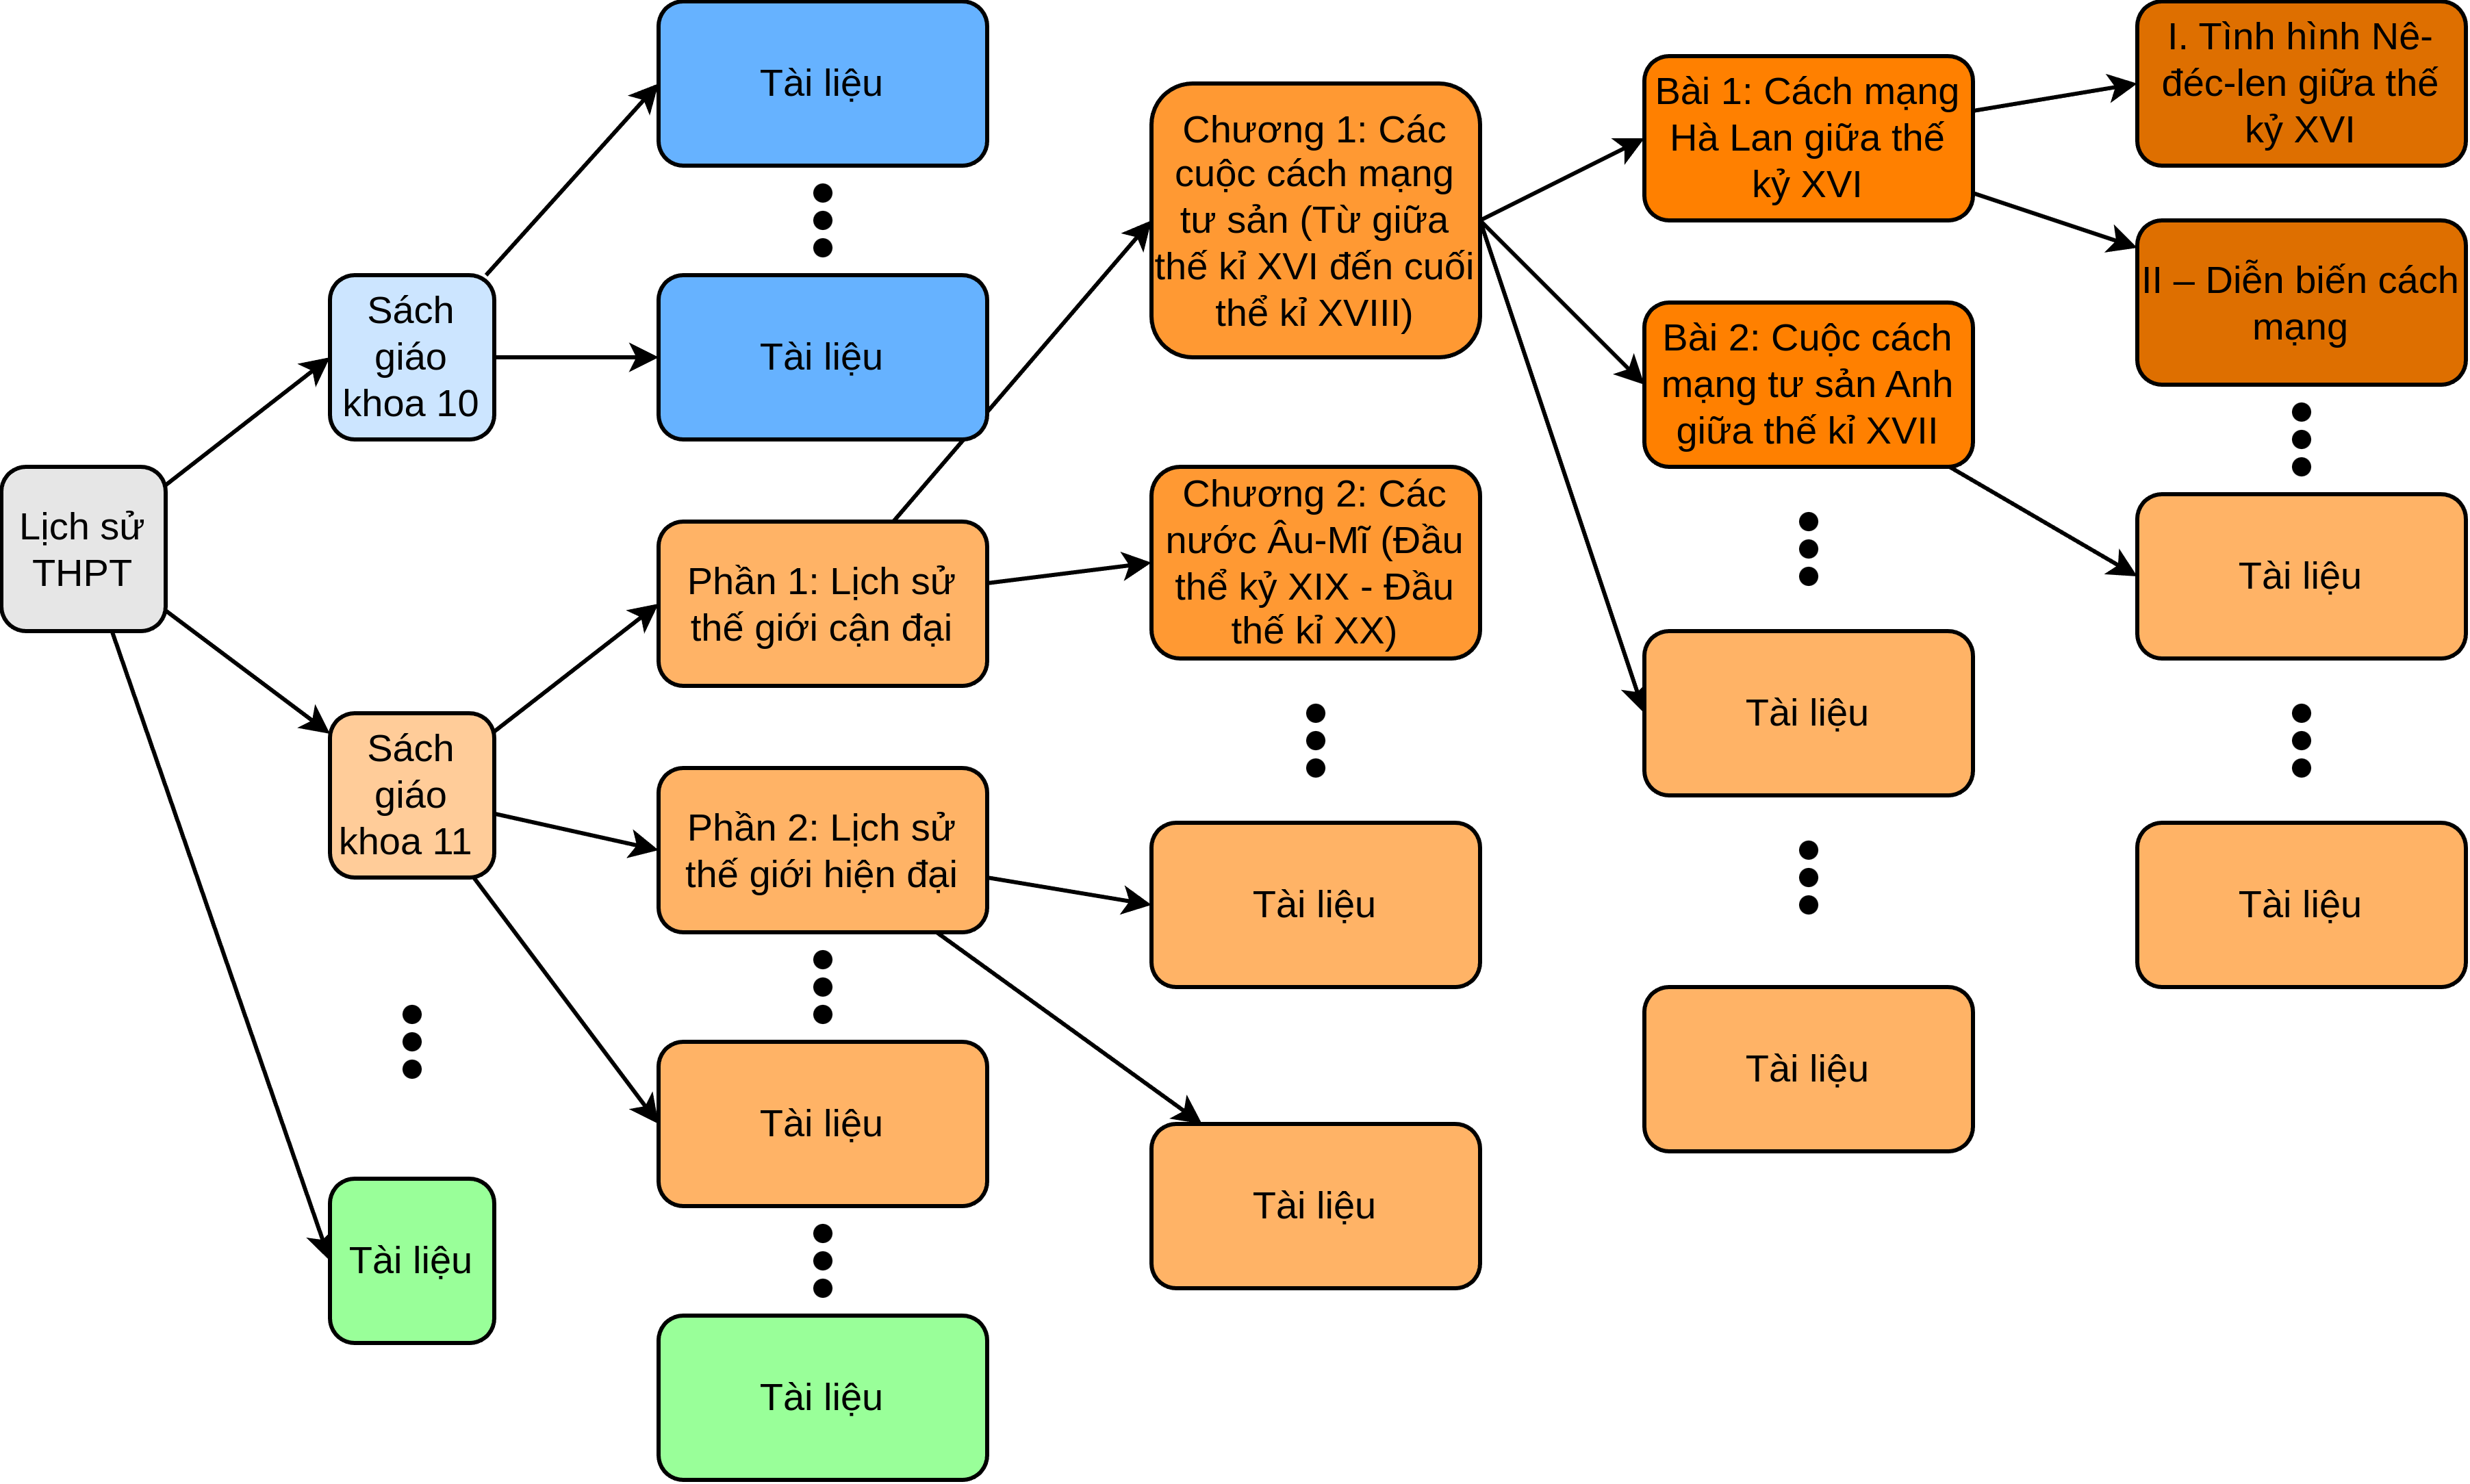
\includegraphics[width=0.8\textwidth]{Chapter4/Fig/document_tree.png}
    \caption{Minh họa cây tài liệu được xây dựng từ bộ tài liệu sách giáo khoa Lịch Sử}
    \label{fig:document_tree}
\end{figure}
\paragraph{Xây dựng đồ thị tri thức:} Vì tài liệu thực nghiệm là lịch sử, vậy nên tôi sẽ trích xuất các thực thể từ các tài liệu thực nghiệm dựa theo ontology được mô tả trong hình \ref{fig:ontology}. Sử dụng phương pháp được nêu tại phần \ref{subsection:knowledge_graph_construction_from_document} Các bước phát hiện thực thể và truy xuất mối quan hệ đều sử dụng mô hình ngôn ngữ lớn GPT-4o với prompt được hiển thị tại phụ lục. Rồi chúng được lưu vào cơ sở dữ liệu đồ thị tri thức Neo4j. Sau khi tri thức là các thực thể và mối quan hệ giữa chúng được lưu vào cơ sở dữ liệu, tôi thực hiện việc cải thiện tri thức để giúp hoàn thiện \gls{kg} và giảm thiểu sai sót với việc cũng sử dụng model GPT-4o để kiểm tra mối quan hệ giữa các thực thể và mối quan hệ.


Kết quả thu được 6600 nút thực thể và 10500 mối quan hệ giữa chúng. Hình \ref{fig:knowledge_graph} mô tả một phần của đồ thị tri thức sau khi xây dựng.
\begin{figure}
    \centering
    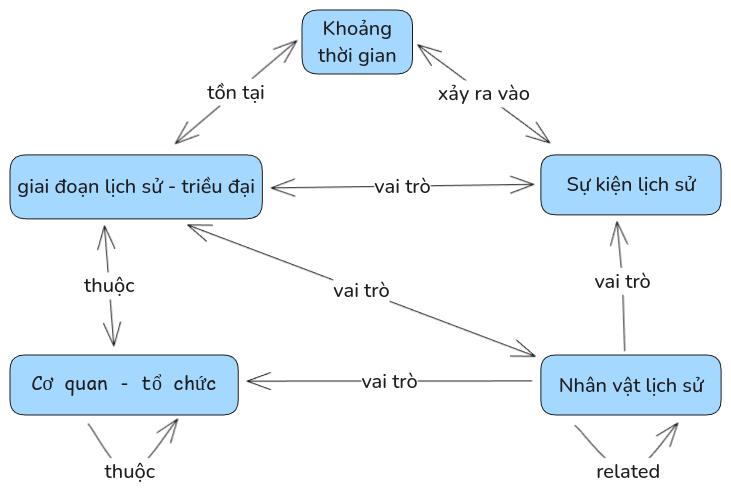
\includegraphics[width=0.75\textwidth]{Chapter4/Fig/ontology.png}
    \caption{Ontology cho lịch sử}
    \label{fig:ontology}
\end{figure}
\begin{figure}
    \centering
    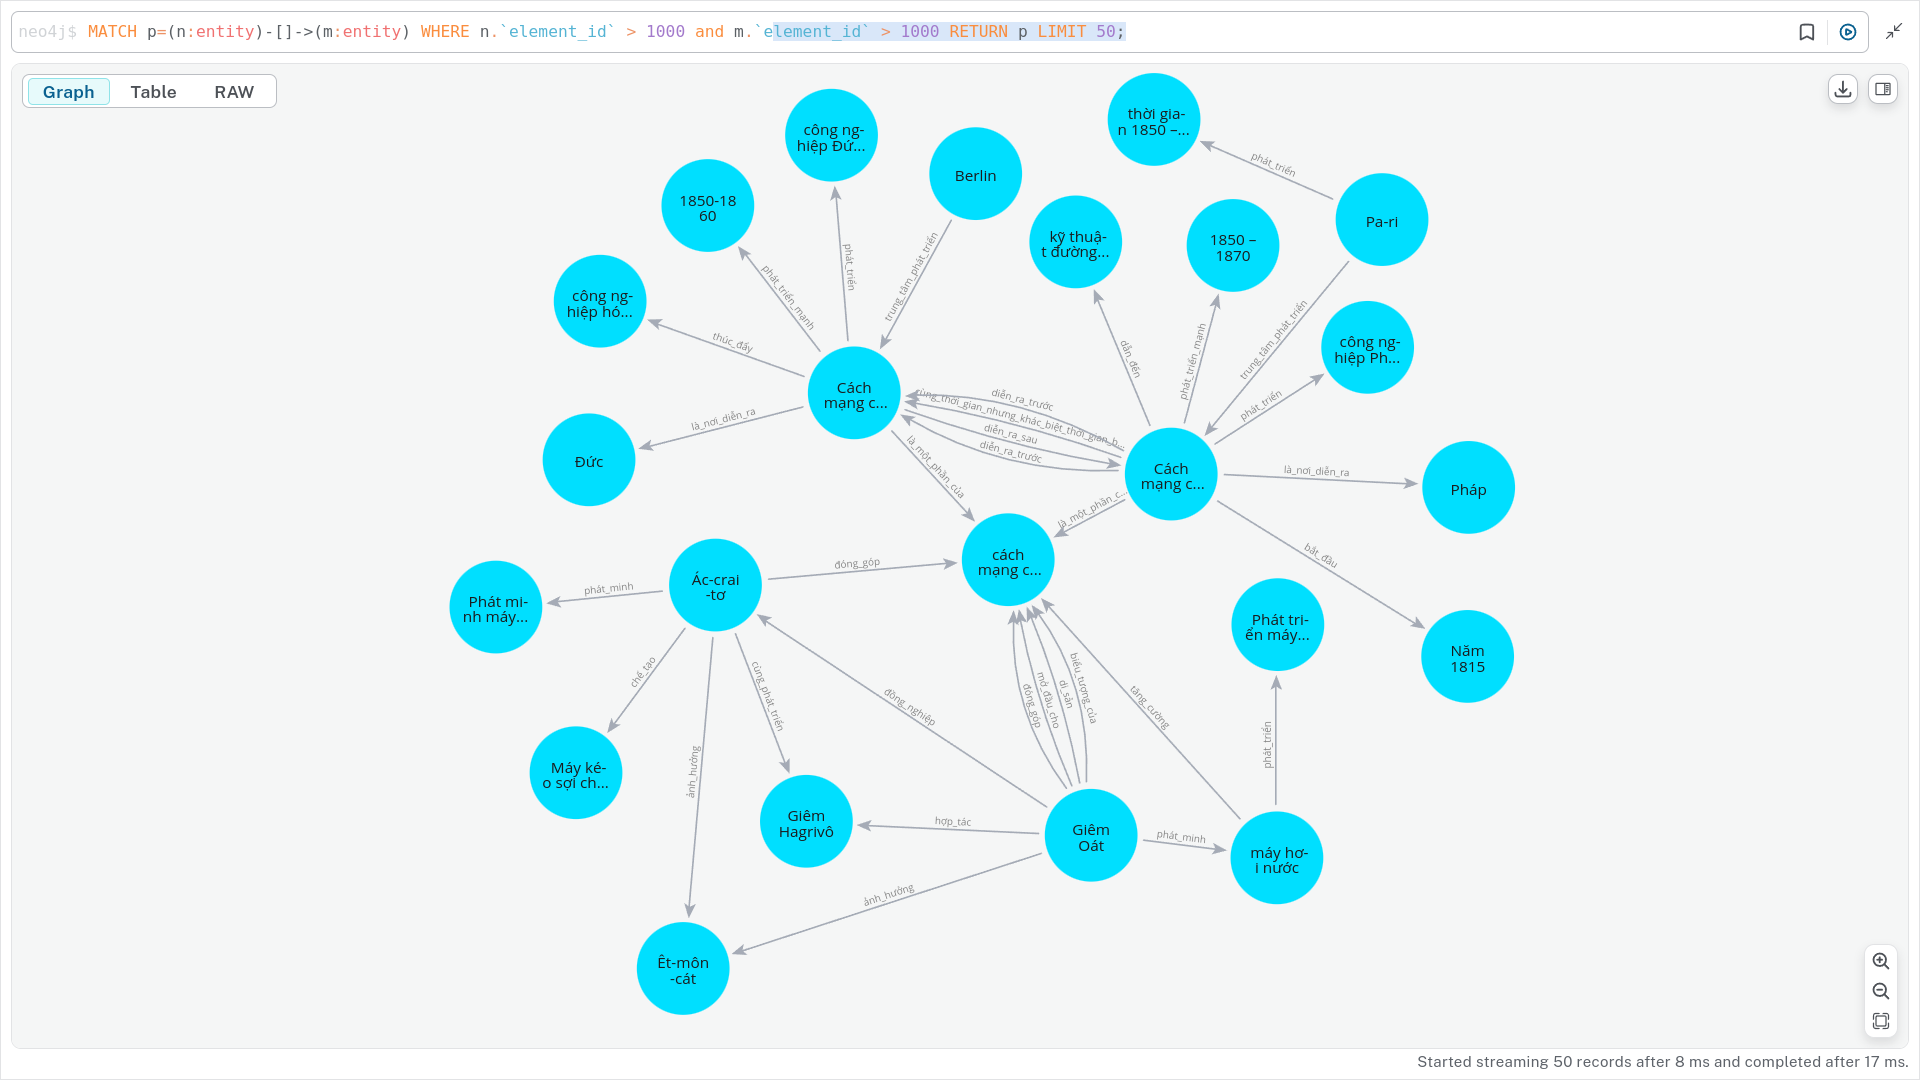
\includegraphics[width=0.8\textwidth, trim=320 50 320 65, clip]{Chapter4/Fig/knowledge_graph.png}
    \caption{Minh họa một phần đồ thị tri thức được xây dựng dựa trên tài liệu sách giáo khoa Lịch Sử}
    \label{fig:knowledge_graph}
\end{figure}


\subsubsection{Xây dựng hệ thống RAG}
\label{section:rag_system_construction_experiment}
Để đánh giá hiệu quả của hệ thống \gls{rag} được đề xuất, tôi đã thiết lập thử nghiệm xây dựng mô hình được đề xuất tại phần \ref{section:rag_integrated_knowledge_graph} với các thành phần chính gồm \gls{llm}, \gls{drms} và các thông số cài đặt.


\paragraph{Mô hình ngôn ngữ lớn} là thành phần chính của mô hình. Trong khóa luận này, tôi chủ yếu sử dụng GPT-4o-mini là \gls{llm} xương sống của mô hình. Do các mô hình này có kích thước lớn và cần tài nguyên phần cứng mạnh mẽ, vậy nên tôi sẽ sử dụng chúng thông qua API từ các dịch vụ cung cấp mô hình như OpenAI API, ... để thực hiện thử nghiệm.


\paragraph{Mô hình truy xuất dày đặc} đóng vai trò quan trọng trong tác vụ đánh giá tài liệu. Trong quá trình thực nghiệm, tôi đã thử nghiệm sử dụng các \gls{drms} khác nhau bao gồm BGE-Embedding, BGE-reranker \cite{BGE_M3_Embedding2024}, Minilm \cite{wang2020minilmdeepselfattentiondistillation}
. Kết quả thực nghiệm cho thấy mô hình BGE-reranker cho kết quả tốt hơn so với các mô hình còn lại, tuy nhiên sẽ gặp vấn đề trong tốc độ tính toán, vậy nên tôi sẽ sử dụng kết hợp cùng mô hình BGE-Embedding để thực hiện thử nghiệm. Do đó, tôi sẽ sử dụng mô hình bge-m3 để chọn ra số lượng lớn các tài liệu phù hợp nhất với câu hỏi và sau đó sử dụng mô hình bge-reranker để xếp hạng lại các tài liệu đó để chọn ra tài liệu phù hợp nhất với câu hỏi (các mô hình \gls{drms} được sử dụng đều là mô hình được đào tạo trước và không có bất kỳ sự tinh chỉnh nào). Vì cả hai mô hình này đều có kích thước nhỏ vậy nên tôi sẽ triển khai chúng trên Colab Pro.


\paragraph{Các thông số cài đặt} của mô hình được đề xuất như sau: tôi đặt tham số temperature của \gls{llm} là 0.4 xuyên xuất quá trình khám phá tri thức và 0 cho quá trình lý luận tri thức. Độ rộng $N=3$ là số lượng đường dẫn truy xuất và số lần tối đa của vòng lặp là 5 để đảm bảo thời gian trả lời của mô hình. Tại bước đánh giá tài liệu, tôi duy trì $k=5$ tài liệu phù hợp nhất với câu hỏi. Tất cả các thông số cài đặt đều được chọn dựa trên kinh nghiệm và thực nghiệm trước đó.
\subsubsection{Giao diện hệ thống}
\label{subsubsection:system_ui}
Để tạo ra một giao diện tương tác với người dùng, tôi đã xây dựng một ứng dụng web demo cho hệ thống được đề xuất. Ứng dụng web demo này sẽ cho phép người dùng nhập câu hỏi và nhận câu trả lời từ hệ thống. Ứng dụng web demo được xây dựng dựa trên mô hình Client-Server, trong đó Server sẽ là hệ thống \gls{rag} được xây dựng và Client sẽ là giao diện người dùng, tuy nhiên trong phạm vi khóa luận này tôi chỉ tập trung vào cải thiện phản hồi của Chatbot. Hệ thống sẽ sử dụng FastAPI để xây dựng API cho hệ thống và NextJS để xây dựng giao diện người dùng. Hình \ref{fig:system_ui} mô tả giao diện người dùng của hệ thống.
\begin{figure}
    \centering
    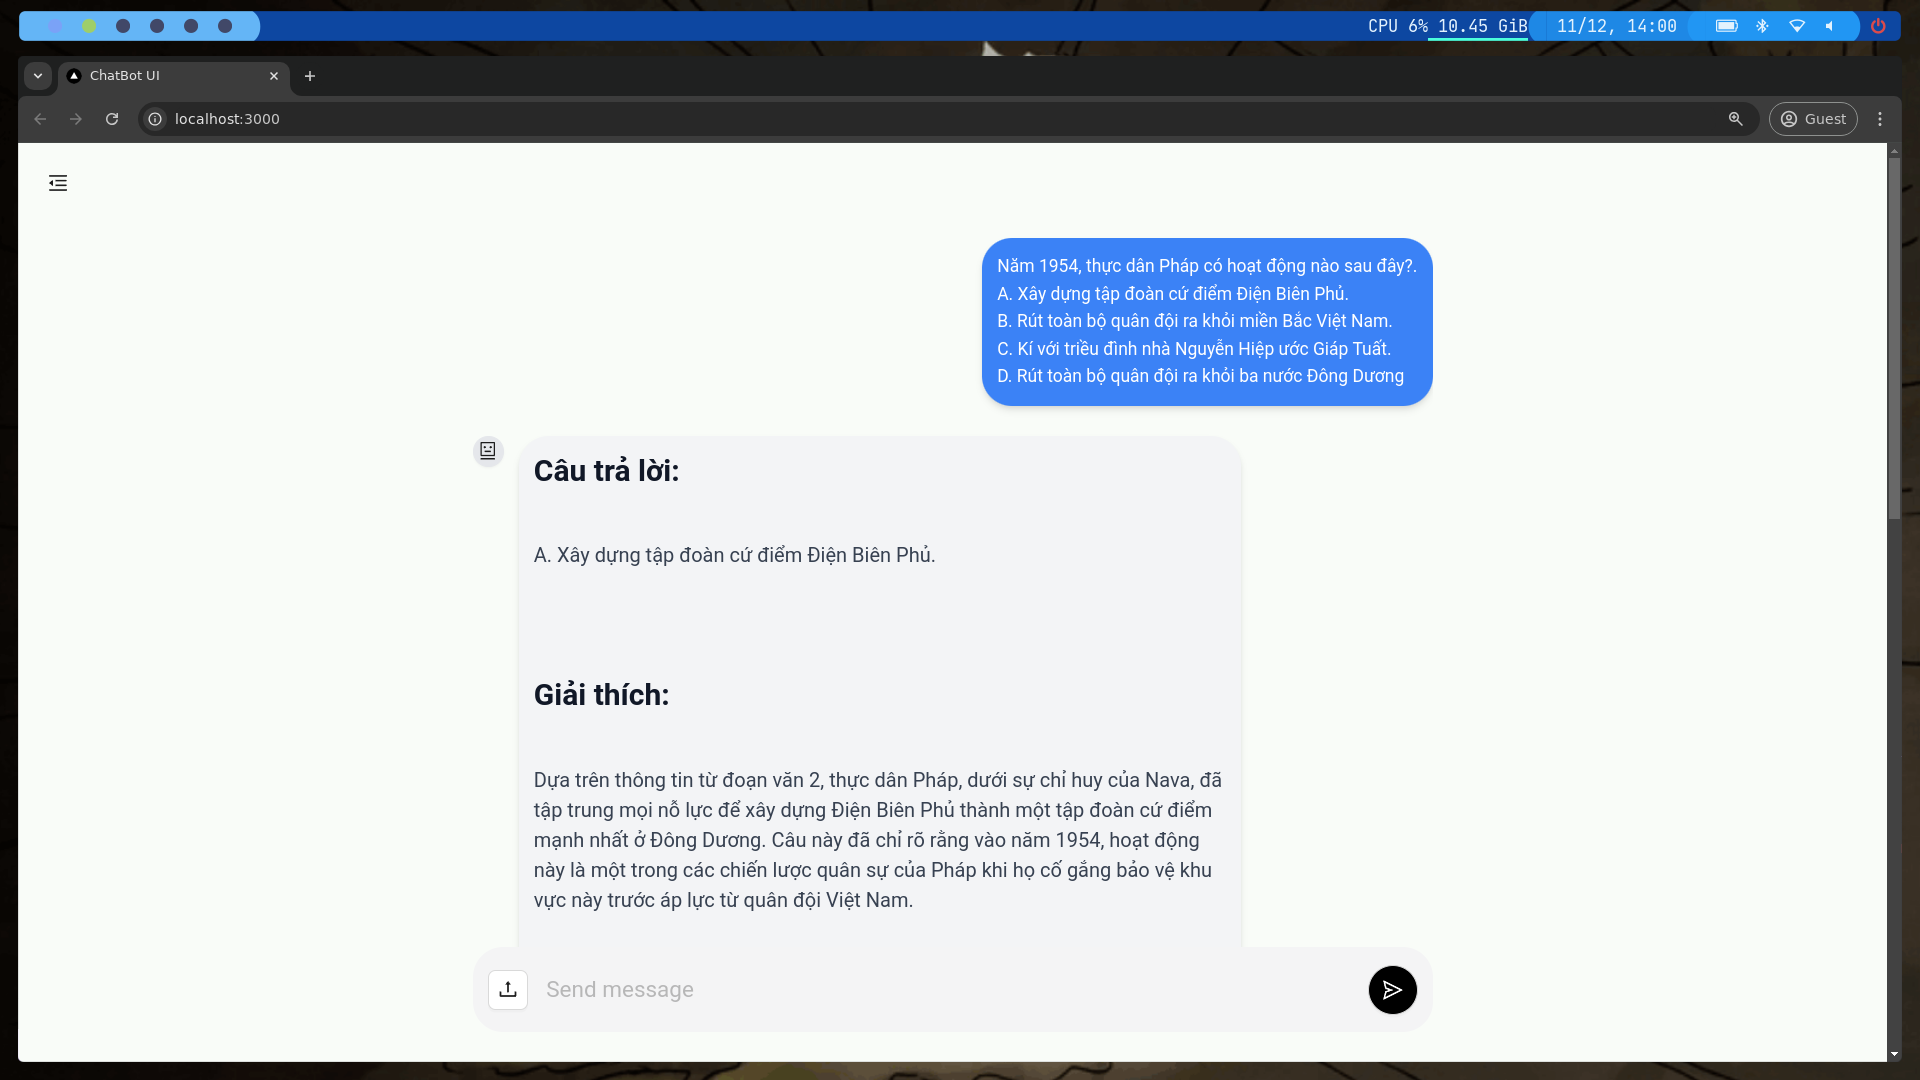
\includegraphics[width=1\textwidth, trim=150 50 150 200, clip]{Chapter4/Fig/system_ui.png}
    \caption{Giao diện người dùng của hệ thống}
    \label{fig:system_ui}
\end{figure}
\subsection{Cài đặt môi trường}
\subsubsection{Phần cứng}
Nghiên cứu sử dụng 2 môi trường phần cứng khác nhau cho các giai đoạn khác nhau:


\begin{table}[ht]
    \centering
    \caption{Cấu hình phần cứng sử dụng trong nghiên cứu}
    \begin{tabular}{|l|l|l|}
        \hline
        \textbf{Môi trường} & \textbf{Cấu hình}     & \textbf{Mục đích sử dụng}     \\ \hline
        Kaggle              & 10 instance với       & Xây dựng đồ thị tri thức      \\
                            & NVIDIA Tesla T4 GPU   &                               \\
                            & (16GB VRAM/instance)  &                               \\ \hline
        Google Colab Pro    & NVIDIA A100-SXM4-40GB & Triển khai hệ thống \gls{rag} \\
                            &                       & chính                         \\ \hline
    \end{tabular}
    \label{tab:hardware}
\end{table}
\subsubsection{Phần mềm}
Dưới đây là danh sách công cụ , thư viện phục vụ cho quá trình huấn luyện và xây dựng ứng dụng dịch máy:


\begin{longtable}{|p{0.25\textwidth}|p{0.15\textwidth}|p{0.5\textwidth}|}
    \caption{Danh sách thư viện và công cụ sử dụng trong nghiên cứu} \label{tab:libraries}                                                              \\


    \hline
    \textbf{Thư viện} & \textbf{Phiên bản} & \textbf{Chức năng}                                                                                         \\ \hline
    \endfirsthead


    % For subsequent pages
    \multicolumn{3}{|c|}{\textit{Tiếp tục từ trang trước}}                                                                                              \\ \hline
    \textbf{Thư viện} & \textbf{Phiên bản} & \textbf{Chức năng}                                                                                         \\ \hline
    \endhead


    \hline
    pandas            & 1.3.3              & Thư viện xử lý dữ liệu dạng bảng, được sử dụng để xử lý dữ liệu thô từ các tài liệu sách giáo khoa Lịch sử \\ \hline
    NumPy             & 1.21.2             & Thư viện xử lý mảng nhiều chiều, được sử dụng để xử lý dữ liệu thô từ các tài liệu sách giáo khoa Lịch sử  \\ \hline
    python-docx       & 1.1.2              & Thư viện xử lý tài liệu Word, được sử dụng để trích xuất dữ liệu từ các tài liệu sách giáo khoa Lịch sử    \\ \hline
    pdfplumber        & 0.11.4             & Thư viện xử lý tài liệu PDF, được sử dụng để trích xuất dữ liệu từ các tài liệu sách giáo khoa Lịch sử     \\ \hline
    Neo4j             & 5.26.0             & Hệ quản trị cơ sở dữ liệu đồ thị, được sử dụng để lưu trữ và truy vấn dữ liệu đồ thị tri thức              \\ \hline
    Huggingface       & 0.23.1             & Thư viện cung cấp các mô hình nhúng, được sử dụng để nhúng câu hỏi và tài liệu văn bản                     \\ \hline
    LangChain         & 0.3.7              & Thư viện cung cấp các mô hình ngôn ngữ lớn, được sử dụng để xây dựng hệ thống \gls{rag}                    \\ \hline
    FastAPI           & 0.115.3            & Framework xây dựng hệ thống API, sử dụng để xây dựng ứng dụng web demo                                     \\ \hline
    NextJS            & 14.0.3             & Framework UI Web, sử dụng để xây dựng giao diện tương tác với người dùng                                   \\ \hline
\end{longtable}




\section{Dữ liệu thực nghiệm}
\label{sec:experiment_data}
\paragraph{Dữ liệu cho việc xây dựng đồ thị tri thức:}
Chúng tôi đã sử dụng để bộ dữ liệu thực nghiệm là bộ sách giáo khoa Lịch Sử. Lịch sử là một đề tài chứa nhiều câu hỏi cần suy luận cũng như kiến thức chuyên ngành. Đây là một lĩnh vực phù hợp để kiểm tra khả năng hiểu ngôn ngữ và truy xuất thông tin của hệ thống chatbot được đề xuất. Các tài liệu sách giáo khoa đều là PDF, vậy nên chúng sẽ được tiền xử lý trước và chỉ trích xuất toàn bộ văn bản có trong các tài liệu đó.
\paragraph{Dữ liệu cho việc đánh giá hệ thống RAG:}
Để đánh giá chất lượng trả lời câu hỏi của hệ thống Chatbot, tôi sẽ sử dụng tập dữ liệu là tập đề thi tốt nghiệp THPT quốc gia môn Lịch sử từ năm 2018 đến 2022 với 4 mã đề khác nhau của từng năm. Đề thi này sẽ có 40 câu hỏi trắc nghiệm với 4 đáp A B C D, trong đó có 1 đáp án đúng duy nhất. Kiến thức của đề và trải dài kiến thức từ cơ bản đến nâng cao, từ đó giúp đánh giá khả năng trả lời câu hỏi của hệ thống Chatbot trong nhiều trường hợp khác nhau. Minh họa đề thi tốt nghiệp THPT quốc gia môn Lịch sử năm 2021 được mô tả trong phần phụ lục \ref{chap:appendix_exam}.


\section{Kết quả thực nghiệm}
\label{section:experiment_results}
Với mỗi đề thi trong tập dữ liệu đề thi tốt nghiệp THPT quốc gia môn Lịch sử, tôi sẽ thử nghiệm trả lời trả lời 10 lần mỗi đề thi và đánh giá trung bình kết quả trả lời của hệ thống. Kết quả trả lời của hệ thống sẽ được đánh giá dựa trên các tiêu chí được nêu tại phần \ref{section:evaluation_metrics}.
\subsection{Chỉ số đánh giá}
\label{section:evaluation_metrics}
Trong phạm vi khóa luận này, tôi sử dụng hai chỉ số chuẩn để đánh giá hệ thống QA: Exact Match (EM) và F1 Score \cite{rajpurkar-etal-2016-squad}. Ngoài ra tôi sử dụng thêm chỉ số Cohen’s Kappa \cite{article_cohens_kappa}, đây là một chỉ số thống kê được sử dụng để đo lường mức độ
thỏa thuận giữa hai bộ phân loại trong các tình huống có thể xảy ra ngẫu nhiên. Không giống như các chỉ số như EM hay F1, Cohen’s Kappa không chỉ tính toán sự tương đồng tuyệt đối mà còn tính đến khả năng thỏa thuận ngẫu nhiên, do đó cung cấp một đánh giá khách quan hơn về hiệu suất của mô hình. Cohen's Kappa cũng hữu ích khi so sánh hiệu suất của các phương pháp khác nhau, chẳng hạn như phương pháp được đề xuất trong khóa luận và các phương pháp truyền thống.


\textbf{Exact Match (EM)} đo lường tỷ lệ phần trăm các dự đoán chính xác khớp với các câu trả lời thực tế. Nó được định nghĩa như sau:


\begin{equation*}
    \text{EM} (\%) = \frac{\lvert \{i \mid \hat{a}_i = a_i \} \rvert}{N} \times 100,
\end{equation*}
trong đó $\hat{a}_i$ là câu trả lời dự đoán, $a_i$ là câu trả lời thực tế, và $N$ là số mẫu.


\textbf{F1 Score} xem xét cả độ chính xác (precision) và độ bao phủ (recall) của các câu trả lời dự đoán, cung cấp một sự cân bằng giữa hai yếu tố này. Điểm F1 cho mỗi trường hợp được tính như sau:
\begin{equation*}
    \text{F1} (\%) = 2 \times \frac{\text{Precision} \times \text{Recall}}{\text{Precision} + \text{Recall}} \times 100.
\end{equation*}
Độ chính xác (precision) và độ bao phủ (recall) được tính dựa trên các từ chung giữa câu trả lời dự đoán và câu trả lời đúng. Điều này đặc biệt hữu ích trong các trường hợp câu trả lời là các cụm từ hoặc câu.


\textbf{Cohen's Kappa} được dùng để đánh giá mức độ đồng thuận giữa hai người đánh giá hoặc giữa hai bộ dữ liệu phân loại. Trong phạm vi khóa luận này, Cohen's Kappa được sử dụng để đo lường mức độ đồng thuận giữa đáp án của mô hình và đáp án của con người. Công thức tính Cohen's Kappa được định nghĩa như sau:
\begin{equation*}
    \kappa = \frac{p_o - p_e}{1 - p_e}
\end{equation*}
Trong đó $p_o$ là tỷ lệ sự thỏa thuận giữa hai bộ phân loại, và $p_e$ là tỷ lệ sự thỏa thuận ngẫu nhiên giữa hai bộ phân loại.


\subsection{Kết quả so sánh với điểm trung bình của học sinh từng năm
}
Để đánh giá hiệu quả của hệ thống \gls{rag} được xây dựng, tôi đã so sánh điểm trung bình của các câu trả lời do hệ thống tạo ra với điểm trung bình thực tế của học sinh từng năm trong kỳ thi THPT Quốc gia môn Lịch sử. Dữ liệu tham khảo từ Bộ Giáo dục và Đào tạo cho thấy điểm trung bình của học sinh dao động trong khoảng từ 4.5 đến 6.0 trên thang điểm 10 trong giai đoạn 2018-2022. Kết quả trung bình do hệ thống \gls{rag} trả lời được thể hiện như hình \ref{fig:evaluation}.
\begin{figure}
    \centering
    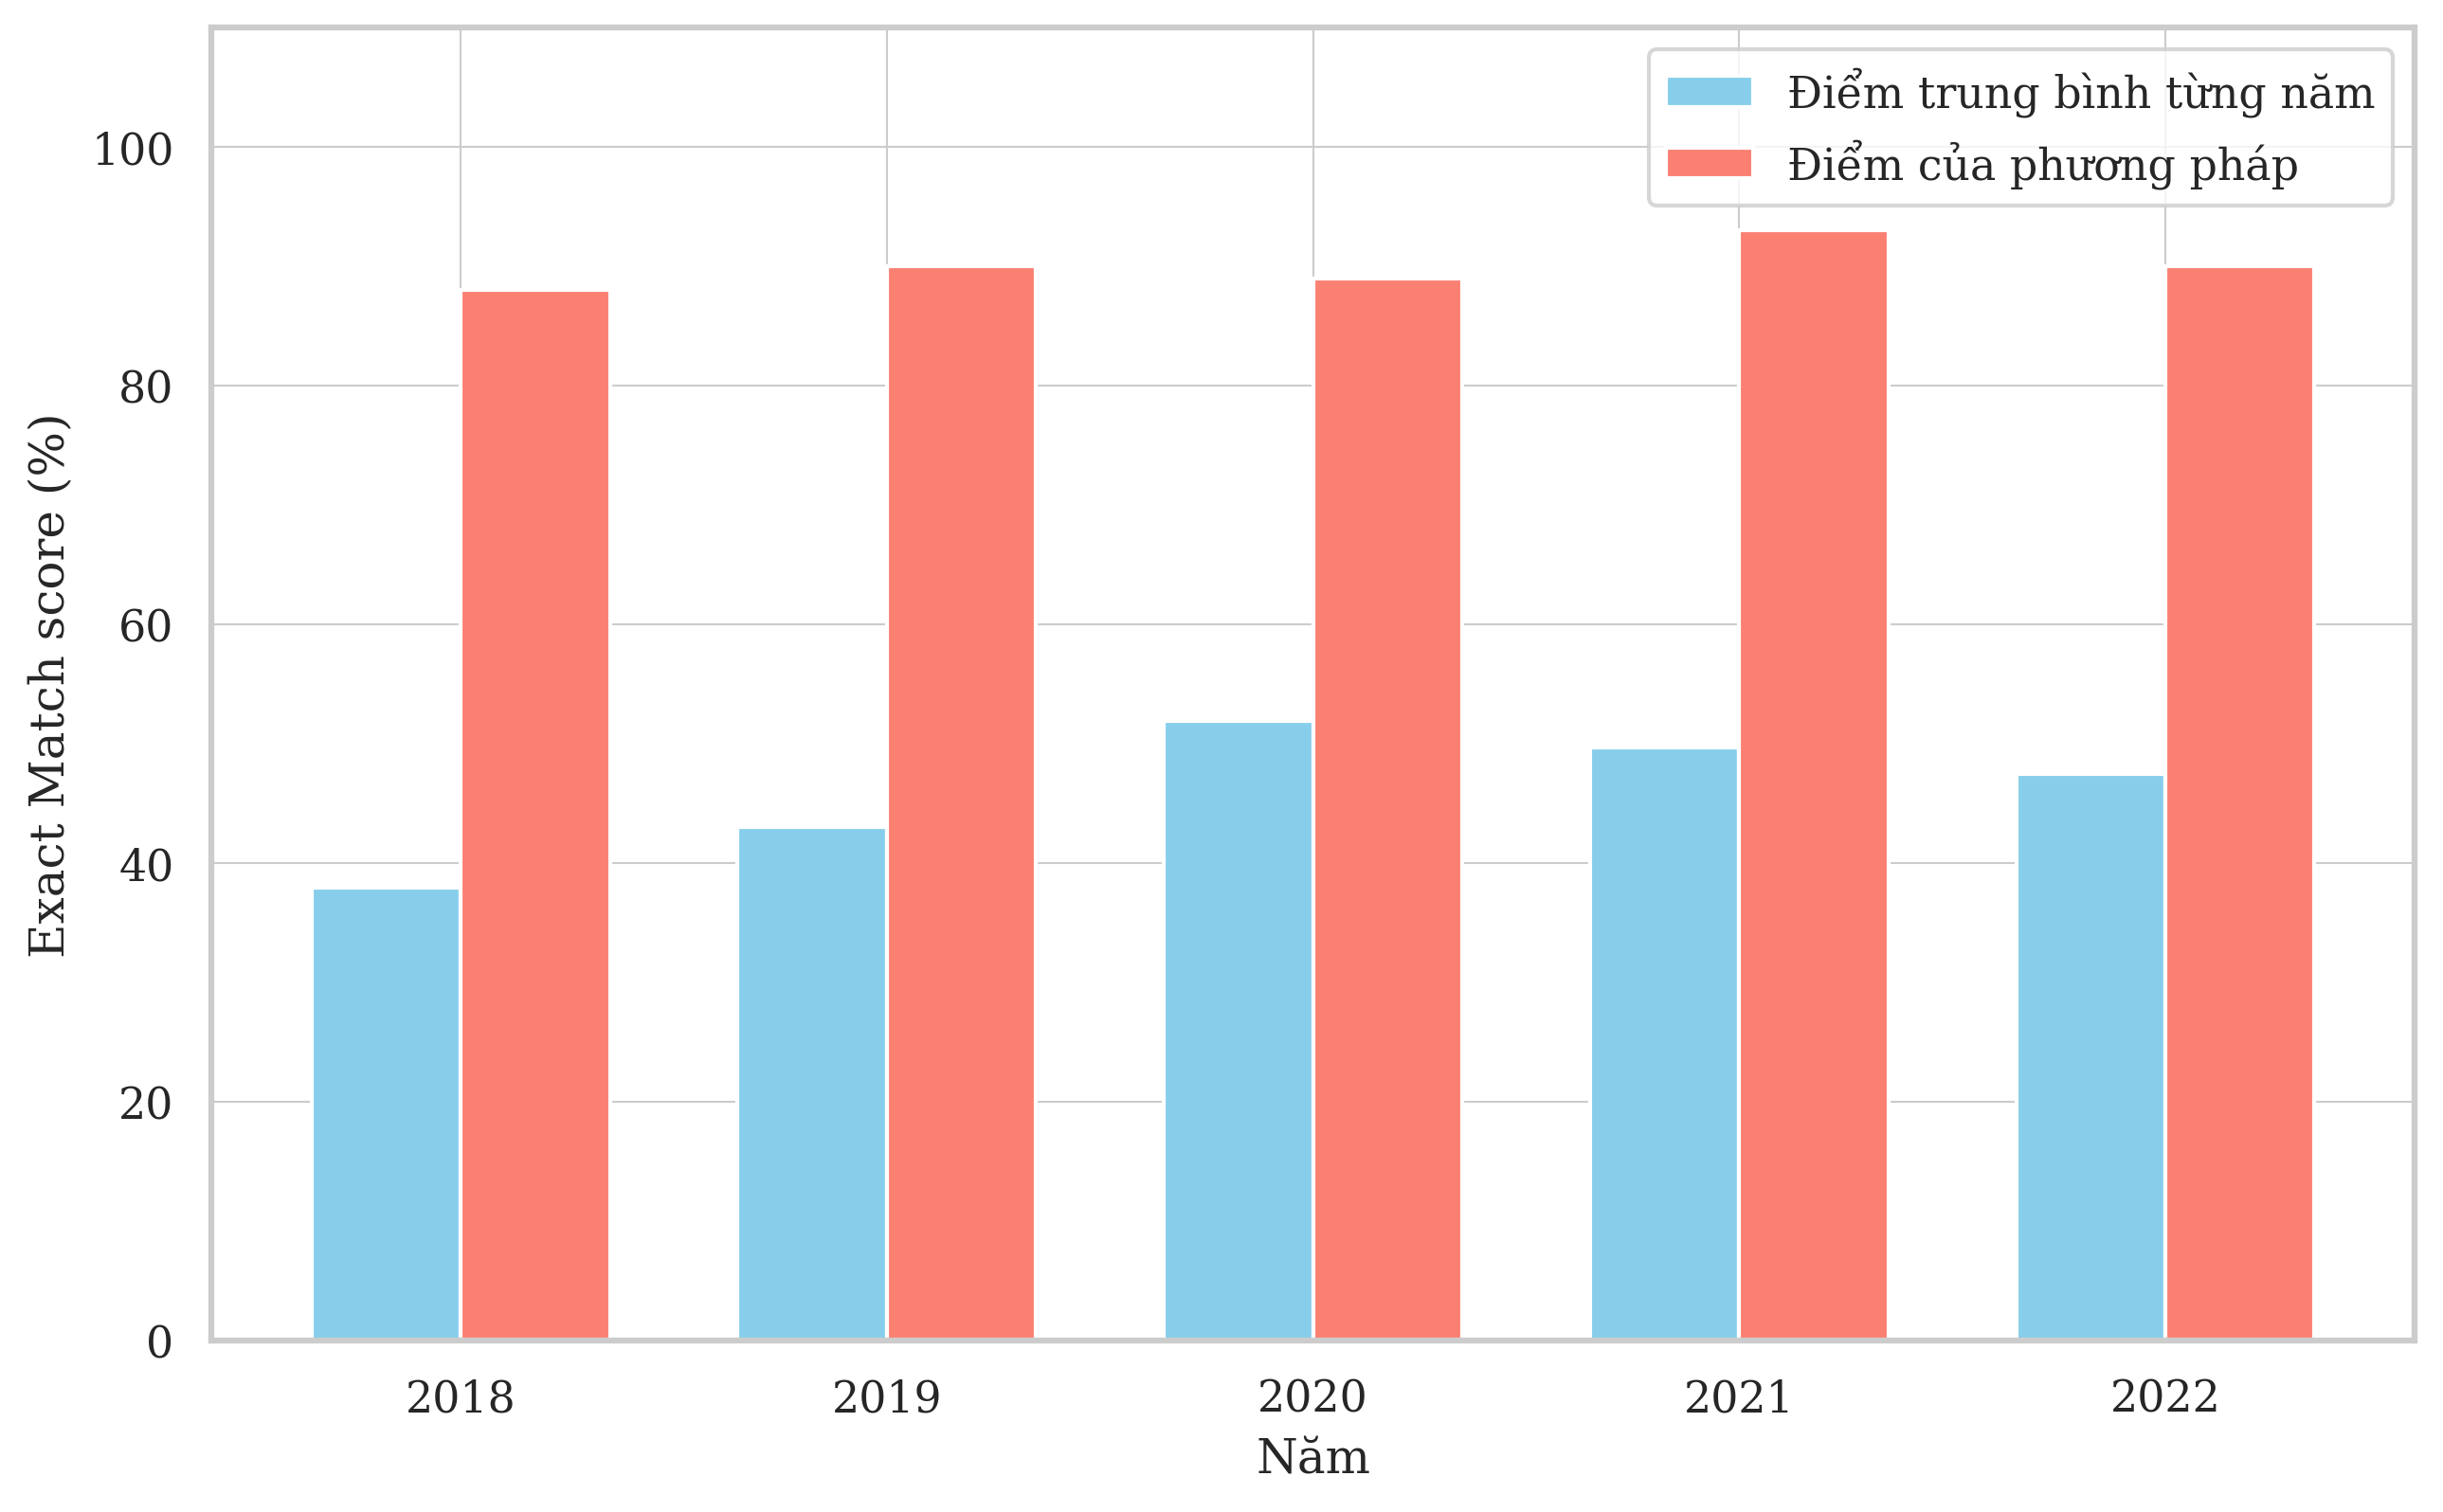
\includegraphics[width=1\textwidth]{Chapter4/Fig/compare_with_average.png}
    \caption{Kết quả so sánh với kết quả trung bình của từng năm}
    \label{fig:evaluation}
\end{figure}


\paragraph{Nhận xét:}


Điểm trung bình từ hệ thống \gls{rag} luôn đạt từ 8.8 đến 9 điểm, mức điểm đòi hỏi sự hiểu biết sâu rộng và kỹ năng suy luận tốt. Điểm số của hệ thống cũng cao tương đối hơn điểm trung bình của học sinh với sự chênh lệch từ 4 đến 5 điểm, cho thấy khả năng hiểu và trả lời câu hỏi tốt hơn phần lớn các thí sinh tham gia kỳ thi. Tổng quan, có thể thấy hệ thống \gls{rag} có khả năng trả lời câu hỏi trắc nghiệm môn Lịch sử với độ chính xác cao và đồng thuận tốt, giúp nâng cao chất lượng phản hồi của chatbot.


\subsection{So sánh với các phương pháp RAG khác}
Tôi đã thiết lập thực nghiệm so sánh với các phương pháp cơ sở khác để cung cấp cái nhìn tổng quan, bao gồm: phương pháp chỉ sử dụng \gls{llm} mà không có tri thức bên ngoài, \gls{rag} truyền thống dựa trên truy xuất văn bản trực tiếp từ tài liệu để trả lời câu hỏi. Bảng \ref{tab:baseline_comparison} trình bày kết quả so sánh:
\begin{table}[ht]
    \centering
    \caption{So sánh hiệu suất của các phương pháp khác nhau với GPT-4o-mini.}
    \small{
        \begin{tabular}{lccc}
            \toprule
            Baseline type  & \multicolumn{3}{c}{Metric}                            \\
            \cmidrule(lr){2-4}
                           & Exact Match                & F1 score & Cohen’s Kappa \\
            \midrule
            LLM directly   & 89.41                      & 89.34    & 85.67         \\
            LLM with CoT   & 90.04                      & 89.95    & 85.89         \\
            Text-based RAG & 82.07                      & 82.13    & 75.89         \\
            Proposed       & 90.93                      & 90.01    & 86.42         \\
            \bottomrule
        \end{tabular}}


    \label{tab:baseline_comparison}
\end{table}
\paragraph{Nhận xét:} kết quả trong Bảng \ref{tab:baseline_comparison} cho thấy phương pháp được đề xuất có hiệu suất vượt trội hơn so với các phương pháp khác ở cả ba chỉ số đánh giá: Exact Match, F1 score, và Cohen’s Kappa. Cụ thể khi so với việc để LLM trực tiếp trả lời, phương pháp đề xuất đã cải thiện 1.52\% (Exact Match), 0.67\% (F1 score) và 0.75 (Cohen’s Kappa). So với LLM sử dụng phương pháp CoT, hiệu suất tăng nhẹ với 0.89\% (Exact Match), 0.06\% (F1 score) và 0.53 (Cohen’s Kappa). Đặc biệt, so với RAG dựa trên truy xuất văn bản, sự cải thiện rõ rệt: 8.86\% (Exact Match), 7.88\% (F1 score), và 10.53 (Cohen’s Kappa), điều này có thể do với các câu hỏi trắc nghiệm chứa nhiều câu hỏi nhiễu, khiến cho việc truy xuất thông tin từ tri thức trở nên khó khăn và RAG truyền thống không thể đáp ứng được.


Nhìn chung, phương pháp đề xuất không chỉ kết hợp hiệu quả các ưu điểm của \gls{llm} và \gls{rag} mà còn cải thiện độ chính xác và sự đồng thuận trong việc trả lời các câu hỏi nói chung và câu hỏi trắc nghiệm nói riêng, làm nổi bật tiềm năng của nó trong việc áp dụng vào các bài toán thực tế.




\subsection{Đánh giá sự tác động của LLMs}
Thêm vào đó để đánh giá tác động của \gls{llm} với khả năng của mô hình, tôi cũng tiến hành thực nghiệm với các \gls{llm} khác bao gồm:
GPT-4o, GPT-4o-mini, Llama3.3-70B, Llama3.1-8B. Kết quả được thể hiện trong bảng \ref{tab:llm_comparison}.
\begin{table}[ht]
    \centering
    \caption{So sánh hiệu suất giữa câu trả lời trực tiếp và phương pháp đề xuất với các mô hình khác nhau. Các giá trị trong ngoặc đơn biểu thị phần trăm cải thiện.}
    \resizebox{\textwidth}{!}{
        \begin{tabular}{lcccccccc}
            \toprule
                          & \multicolumn{2}{c}{GPT-4o} & \multicolumn{2}{c}{GPT-4o-mini} & \multicolumn{2}{c}{Llama3.3-70B} & \multicolumn{2}{c}{Llama3.1-8B}                                                                          \\
            \cmidrule(lr){2-3} \cmidrule(lr){4-5} \cmidrule(lr){6-7} \cmidrule(lr){8-9}
                          & Direct                     & Proposed                        & Direct                           & Proposed                        & Direct & Proposed                 & Direct & Proposed                  \\
            \midrule
            Exact Match   & 89.65                      & 91.37 ($\uparrow$ 1.9\%)        & 89.41                            & 90.93 ($\uparrow$ 1.7\%)        & 77.53  & 79.13 ($\uparrow$ 2.1\%) & 60.58  & 68.43 ($\uparrow$ 12.9\%) \\
            F1 Score      & 89.62                      & 90.92 ($\uparrow$ 1.5\%)        & 89.34                            & 90.01 ($\uparrow$ 0.8\%)        & 78.44  & 79.45 ($\uparrow$ 1.3\%) & 60.21  & 67.28 ($\uparrow$ 11.7\%) \\
            Cohen’s Kappa & 85.99                      & 86.42 ($\uparrow$ 0.5\%)        & 85.67                            & 86.14 ($\uparrow$ 0.6\%)        & 69.81  & 72.78 ($\uparrow$ 4.3\%) & 47.26  & 56.86 ($\uparrow$ 20.3\%) \\
            \bottomrule
        \end{tabular}}

    \label{tab:llm_comparison}
\end{table}
\paragraph{Nhận xét:}bảng \ref{tab:llm_comparison} cho thấy tác động tích cực của phương pháp đề xuất đối với hiệu suất của các mô hình ngôn ngữ lớn (LLMs). Cụ thể:
\begin{itemize}
    \item \textbf{Tăng cường hiệu suất tổng thể} khi các chỉ số đánh giá  Exact Match, F1 Score, và Cohen’s Kappa đều cải thiện dù là cải thiện nhẹ khi sử dụng phương pháp đề xuất so với câu trả lời trực tiếp trên tất cả các mô hình. Cụ thể khi sử dụng mô hình lớn là GPT-4o, GPT-4o-mini kết quả tăng khoảng 1.4\%, trong khi đó với các mô hình nhỏ hơn mang lại kết quả tốt hơn khoảng 7-9\%.
    \item \textbf{Khả năng cải thiện khác biệt giữa các mô hình:} Các mô hình lớn hơn như GPT-4o, GPT-4o-mini, Llama3.3-70B cho thấy sự cải thiện khiêm tốn hơn so với ,điều này có thể đo mức độ phức tạp và khả năng biểu diễn vốn đã rất cao của các mô hình lớn. Nhưng với Llama3.1-8B, mức độ cải thiện rõ rệt hơn (Exact Match tăng từ 60.58\% lên 68.43\% và F1 Score từ 60.21\% lên 67.28\%). Điều này chỉ ra rằng các mô hình nhỏ hơn có tiềm năng được cải thiện đáng kể nhờ phương pháp đề xuất.
\end{itemize}
Từ kết quả trên có thể thấy phương pháp đề xuất đã thể hiện khả năng cải thiện đáng kể hiệu suất của các LLMs, đặc biệt đối với các mô hình nhỏ hoặc trung bình.
\subsection{Đánh giá khả năng trả lời câu hỏi và đưa ra giải thích}
Ngoài các đánh giá dựa trên sự chính xác của đáp án trắc nghiệm, tôi cũng đã thực hiện đánh giá khả năng của hệ thống trong việc trả lời câu hỏi mở và đưa ra giải thích cho câu trả lời. Kết quả các thực nghiệm được thể hiện trong các bảng \ref{tab:open_question}, \ref{tab:open_question_2}, và \ref{tab:mcp_question}.


\begin{table}[ht]
    \centering
    \caption{Thực nghiệm trả lời câu hỏi mở.}
    \resizebox{1\textwidth}{!}{
        \scriptsize{
            \begin{tabular}{|p{3cm}|p{10cm}|}
                \hline
                \textbf{Câu hỏi}     & Quốc gia nào phát động Chiến tranh lạnh chống Liên Xô?                                                                                                                                                                                                                                                                                                                                                                                                                                                                                                                                       \\
                \hline
                \textbf{Câu trả lời} & \textbf{Câu trả lời:} Quốc gia phát động Chiến tranh lạnh chống Liên Xô là Mỹ.                                                                                                                                                                                                                                                                                                                                                                                                                                                                                                               \\
                                     & \textbf{Giải thích:}                                                                                                                                                                                                                                                                                                                                                                                                                                                                                                                                                                         \\
                                     & Căn cứ vào các đoạn văn đã cung cấp, đặc biệt từ đoạn 1, có thể thấy rõ rằng sau Chiến tranh thế giới thứ hai, mối quan hệ giữa Liên Xô và Mỹ đã nhanh chóng chuyển từ liên minh chống phát xít sang đối đầu. Trong đoạn 1, thông điệp của Tổng thống Truman vào ngày 12-3-1947 được nhấn mạnh như là khởi đầu cho chính sách chống Liên Xô của Mỹ, được gọi là "Học thuyết Truman". Điều này cho thấy Mỹ đã chủ động phát động chính sách chiến tranh lạnh để chống lại Liên Xô, với ý định ngăn chặn sự lan rộng của chủ nghĩa xã hội và tăng cường ảnh hưởng của mình trên toàn thế giới. \\


                                     & Bên cạnh đó, trong đoạn 5, có đề cập đến việc các nước Tây phương do Mỹ lãnh đạo đã theo đuổi chính sách chống cộng và tiến hành Chiến tranh lạnh, điều này càng củng cố cho luận điểm rằng Mỹ là quốc gia phát động chiến tranh lạnh chống Liên Xô.                                                                                                                                                                                                                                                                                                                                         \\


                                     & Do đó, câu trả lời là Mỹ là quốc gia phát động Chiến tranh lạnh chống Liên Xô.                                                                                                                                                                                                                                                                                                                                                                                                                                                                                                               \\
                \hline
                \textbf{Đáp án}      & Mỹ                                                                                                                                                                                                                                                                                                                                                                                                                                                                                                                                                                                           \\
                \hline
            \end{tabular}
        }
    }
    \label{tab:open_question}
\end{table}
\begin{table}[ht]
    \centering
    \caption{Thực nghiệm trả lời câu hỏi mở.}
    \resizebox{1\textwidth}{!}{
        \scriptsize{\begin{tabular}{|p{3cm}|p{10cm}|}
                \hline
                \textbf{Question}    & Sự phát triển thịnh đạt của các quốc gia phong kiến ở Đông Nam Á thế kỉ X-XVIII được biểu hiện như thế nào?                                                                                                                                                                                       \\
                \hline
                \textbf{Câu trả lời} & \textbf{Câu trả lời:} Sự phát triển thịnh đạt của các quốc gia phong kiến ở Đông Nam Á từ thế kỷ X đến XVIII được biểu hiện qua việc hình thành và phát triển của nhiều quốc gia phong kiến mạnh mẽ, sự tiến bộ của nền kinh tế và văn hóa, cũng như việc xây dựng những vùng kinh tế quan trọng.


                \textbf{Giải thích:}


                1. Hình thành quốc gia phong kiến mạnh mẽ: Trong khoảng thời gian này, nhiều quốc gia phong kiến lớn đã hình thành và củng cố quyền lực, như Vương quốc Cam-pu-chia, Đại Việt, Champa, và Vương quốc Pa-gan (Mi-an-ma). Các quốc gia này đã thực hiện các cuộc chinh phục và thống nhất các lãnh thổ nhỏ hơn, gia tăng quyền lực và sự giàu có.


                2. Phát triển kinh tế: Kinh tế khu vực phát triển thịnh vượng với sản xuất nông nghiệp lớn, bao gồm lúa gạo và các sản phẩm thủ công như vải, đồ sứ... Sự phát triển này tạo ra khả năng cung cấp sản phẩm quý giá cho thị trường thế giới, thu hút thương nhân từ nhiều quốc gia đến giao thương.


                3. Xây dựng văn hóa dân tộc: Đi cùng sự phát triển kinh tế là sự hình thành và phát triển văn hóa của các dân tộc Đông Nam Á, với việc tiếp thu và sáng tạo trên nền tảng văn hóa Ấn Độ. Điều này cho thấy sự phát triển không chỉ ở mặt kinh tế mà còn cả ở mặt văn hóa, hình thành nền văn hóa riêng của từng quốc gia.


                Tổng hợp lại, sự phát triển thịnh đạt của các quốc gia phong kiến ở Đông Nam Á từ thế kỷ X đến XVIII thể hiện qua cả yếu tố chính trị, kinh tế và văn hóa, với những quốc gia lớn mạnh và các hoạt động giao thương sôi nổi.                                                                                             \\
                \hline
                \textbf{Đáp án}      & Thế kỉ X-XVIII là thời kỳ thịnh vượng của các quốc gia phong kiến Đông Nam Á, thể hiện qua ba lĩnh vực chính:
                \begin{itemize}
                    \item Chính trị: Sự hình thành và phát triển của nhiều quốc gia phong kiến, như Vương triều Mô-giô-pa-hit ở In-đô-nê-xi-a, Đại Việt dưới các triều Lý, Trần, Lê sơ, Vương quốc Ăng-co của Campuchia, quốc gia Pa-gan ở Mi-an-ma, Vương quốc Su-khô-thay ở lưu vực sông Mê Nam và Vương quốc Lan Xang ở sông Mê Công.
                    \item Kinh tế: Sự phát triển mạnh mẽ của các nền kinh tế, hình thành các vùng kinh tế quan trọng cung cấp lúa gạo, cá, sản phẩm thủ công và tài nguyên thiên nhiên. Đông Nam Á trở thành điểm giao thương của các lái buôn quốc tế.
                    \item Văn hóa: Nền văn hóa dân tộc được hình thành, đóng góp vào kho tàng văn hóa chung của nhân loại.
                \end{itemize}      \\
                \hline
            \end{tabular}}
    }
    \label{tab:open_question_2}
\end{table}
\begin{table}[ht]
    \centering
    \caption{Thực nghiệm lý giải câu hỏi trắc nghiệm.}
    \resizebox{1\textwidth}{!}{
        \scriptsize{\begin{tabular}{|p{3cm}|p{10cm}|}
                \hline
                \textbf{Câu hỏi}     &
                Thế kỉ X – XII, ở khu vực Đông Nam Á, Campuchia được gọi là


                A. vương quốc phát triển nhất.


                B. vương quốc hùng mạnh nhất.


                C. vương quốc mạnh và ham chiến trận nhất.


                D. vương quốc chịu ảnh hưởng sâu sắc nhất của văn hóa Ấn Độ.                                                                                                                                                                                                               \\
                \hline
                \textbf{Câu trả lời} & \textbf{Câu trả lời:} Thế kỷ X – XII, ở khu vực Đông Nam Á, Campuchia được gọi là C. vương quốc mạnh và ham chiến trận nhất.


                \textbf{Giải thích:} Dựa trên đoạn văn thứ nhất, thông tin cho thấy "trong các thế kỷ X – XII, Cam-pu-chia trở thành một trong những vương quốc mạnh và ham chiến trận nhất Đông Nam Á." Từ đây, ta có thể suy ra rằng trong thời kỳ này, Campuchia không chỉ mạnh mẽ mà còn có sự tham gia tích cực trong các hoạt động chiến tranh, bao gồm cả việc chinh phục lãnh thổ của các quốc gia khác.


                \textbf{Phân tích các lựa chọn còn lại:}
                \begin{itemize}
                    \item A. vương quốc phát triển nhất. - Mặc dù Campuchia phát triển nhưng không thể khẳng định nó là "phát triển nhất" trong toàn khu vực.
                    \item B. vương quốc hùng mạnh nhất. - Mặc dầu Campuchia mạnh mẽ, từ thông tin đề cập, từ "hùng mạnh nhất" có thể hiểu là thuộc về lĩnh vực quân sự, không nhất thiết là mạnh nhất tổng thể trong mọi khía cạnh.
                    \item D. vương quốc chịu ảnh hưởng sâu sắc nhất của văn hóa Ấn Độ. - Mặc dù văn hóa Ấn Độ có ảnh hưởng lớn đến các vương quốc Đông Nam Á, không có thông tin rõ ràng chứng minh Campuchia là vương quốc chịu ảnh hưởng sâu sắc nhất so với các quốc gia khác trong khu vực.
                \end{itemize} \\
                \hline
                \textbf{Đáp án}      & C. vương quốc mạnh và ham chiến trận nhất.                                                                                                                                                                                                          \\
                \hline
            \end{tabular}}
    }
    \label{tab:mcp_question}
\end{table}
\paragraph{Nhận xét:} Từ kết quả của các thực nghiệm trên, có thể thấy khả năng trả lời các câu hỏi mở và đưa ra giải thích của hệ thống đề xuất là khá tốt. Cụ thể, hệ thống đã trả lời chính xác và cung cấp các đoạn văn liên quan đối với các câu hỏi tự luận với độ chính xác của quá trình trích xuất thông tin từ tri thức đạt trên 90\%. Đối với các câu hỏi trắc nghiệm, hệ thống cũng đã trả lời chính xác và cung cấp giải thích cho đáp án đúng và lý do các đáp án còn lại sai. Điều này cho thấy hệ thống không chỉ có khả năng trả lời câu hỏi mà còn có khả năng giải thích câu trả lời, giúp người dùng hiểu rõ hơn và tin tưởng hơn vào câu trả lời của hệ thống.